\section{Generalization}

\subsection{Explicit Regularization}

\begin{frame}{The Problem: A Model That Memorizes}
    \frametitle{Overfitting and the Failure to Generalize}
    \begin{itemize}
        \item A model that performs perfectly on training data but fails on new, unseen data has \textbf{overfitted}.
        \item It's like a student who memorizes the answers to past exams but hasn't learned the underlying concepts.
        \item This "generalization gap" is what we aim to reduce.
    \end{itemize}
    \begin{figure}
        % Placeholder for the overfitting graph from Regularization.pdf, p. 5
        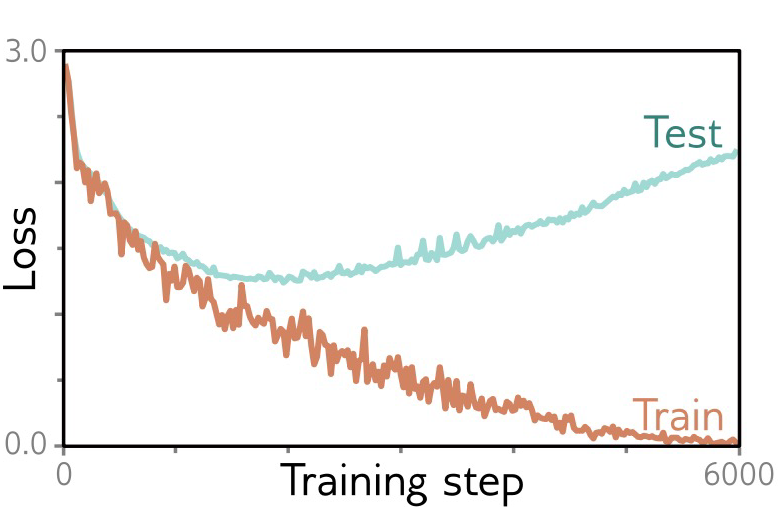
\includegraphics[width=0.7\textwidth]{images/generalization_gap.png}
        \caption{A classic sign of overfitting: training error continues to decrease while test (validation) error begins to rise.}
    \end{figure}
\end{frame}

\begin{frame}{The Solution: A Penalty for Complexity}
    \frametitle{Introducing Regularization}
    How do we encourage our model to learn the true underlying pattern instead of just memorizing the data points?
    \begin{itemize}
        \item We can add a \bhighlight{penalty term} $R(W)$ to our loss function.
        \item This penalty discourages the model from becoming too complex.
        \item Our new objective is to balance two competing goals:
            \begin{enumerate}
                \item Fit the training data well (minimize the original loss).
                \item Keep the model simple (minimize the regularization penalty).
            \end{enumerate}
        \item The new cost function is:
            $$ J(W) = \underbrace{\sum_{n=1}^{N}\text{loss}(y^{(n)}, f(x^{(n)}; W))}_{\text{Data Fit}} + \underbrace{\lambda R(W)}_{\text{Complexity Penalty}} $$
    \end{itemize}
\end{frame}

\begin{frame}{L2 Regularization (Weight Decay)}
    \frametitle{L2 Regularization (Weight Decay)}
    L2 regularization penalizes the squared magnitude of the weights. It encourages the network to use small weights.
    \begin{itemize}
        \item The penalty term is the squared L2 norm of the weights:
            $$ R(W) = ||W||_2^2 = \sum_k \sum_l W_{k,l}^2 $$
        \item The new cost function becomes:
            $$ J(W) = \text{Loss}(W) + \lambda ||W||_2^2 $$
        \item This leads to a modified gradient update rule called \textbf{Weight Decay}:
            $$ W \leftarrow W - \alpha \nabla_W \text{Loss}(W) - 2\lambda W $$
            $$ W \leftarrow (1 - 2\lambda)W - \alpha \nabla_W \text{Loss}(W) $$
        \item At each step, the weights are multiplicatively shrunk before the gradient update.
    \end{itemize}
\end{frame}

\begin{frame}{The Intuition Behind L2 Regularization}
    \frametitle{Why Do Smaller Weights Generalize Better?}
    \begin{itemize}
        \item \textbf{Smoother Functions:} Penalizing large weights forces the network to learn smoother, less complex functions.
        \item \textbf{Linear Regime:} With tanh or sigmoid activations, small weights keep neurons in their linear range. Since linear neurons can only learn simple linear functions, L2 regularization promotes this low-complexity behavior.
    \end{itemize}
    \begin{figure}
        % Placeholder for the sigmoid visualization from Regularization.pdf, p. 14
        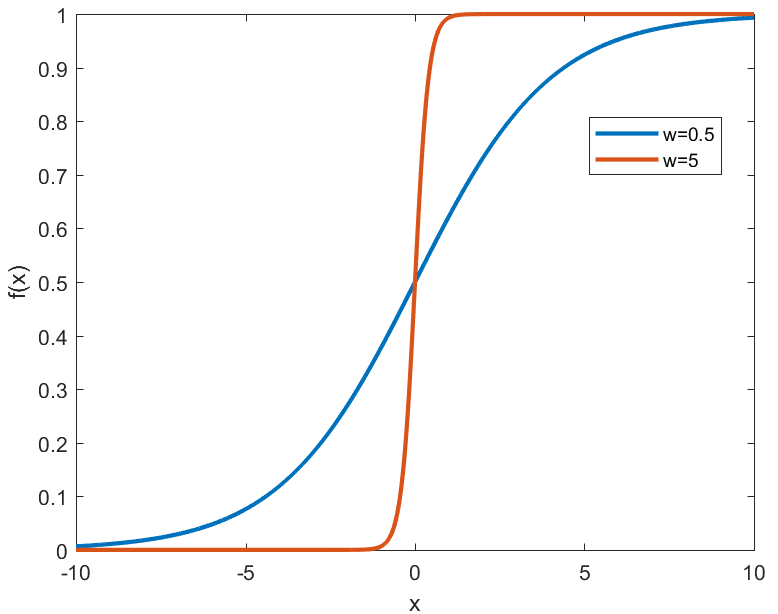
\includegraphics[width=0.5\textwidth]{images/sigmoid_l2.png}
        \caption{As weight `w` increases, the sigmoid function becomes much steeper and more non-linear, allowing for more complex responses.}
    \end{figure}
\end{frame}

\begin{frame}{The Effect of the Regularization Strength $\lambda$}
    \frametitle{Finding the Right Balance}
    The hyperparameter $\lambda$ controls the trade-off between fitting the data and keeping the weights small.
    \begin{figure}
        % Placeholder for the lambda effect visualization from Regularization.pdf, p. 11
        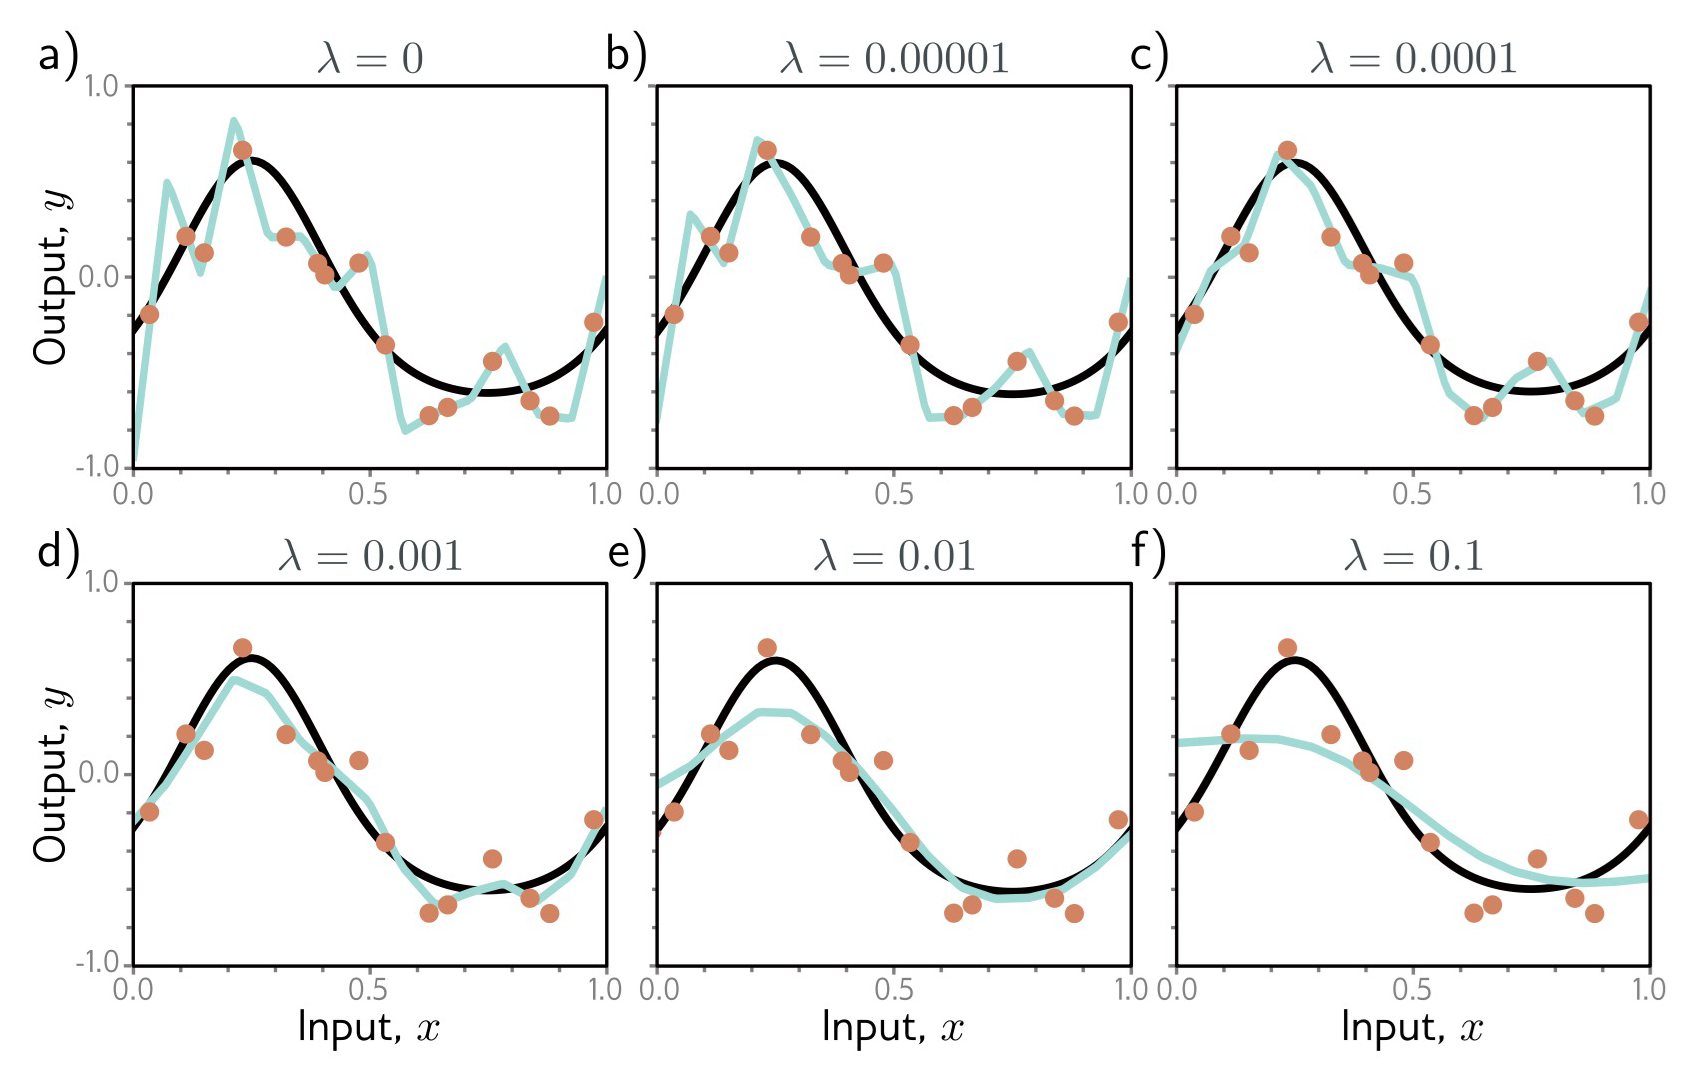
\includegraphics[width=0.9\textwidth]{images/lambda_effect.png}
        \caption{As $\lambda$ increases, the learned function becomes smoother and less prone to overfitting, but too high a value can lead to underfitting.}
    \end{figure}
\end{frame}

\begin{frame}{Geometric Intuition of regularizations}
    L1 regularization penalizes the absolute value of the weights.
    \begin{itemize}
        \item The penalty term is the L1 norm of the weights:
            $$ R(W) = ||W||_1 = \sum_k \sum_l |W_{k,l}| $$
        \item \textbf{Key Property:} L1 regularization is known for producing \bhighlight{sparse weight} vectors. It encourages many weights to be exactly zero.
        \item This can be interpreted as a form of automatic feature selection, as the network learns to ignore irrelevant inputs.
    \end{itemize}
    \begin{alertblock}{L1 vs. L2}
        Use L2 regularization as a default. L1 can be useful if you suspect many of your input features are irrelevant and you want a sparse, more interpretable model.
    \end{alertblock}
\end{frame}

\begin{frame}{Geometric intuition of regularizations}
    \begin{columns}
        \begin{column}{0.5\textwidth}
            \textbf{L2 Regularization}
            \begin{itemize}
                \item Circular constraint
                \item Smooth shrinkage
            \end{itemize}
        \end{column}
        \begin{column}{0.5\textwidth}
            \textbf{L1 Regularization}
            \begin{itemize}
                \item Diamond constraint
                \item Corners hit first
            \end{itemize}
        \end{column}
    \end{columns}

    \vspace{1em}

    \begin{figure}
        \centering
        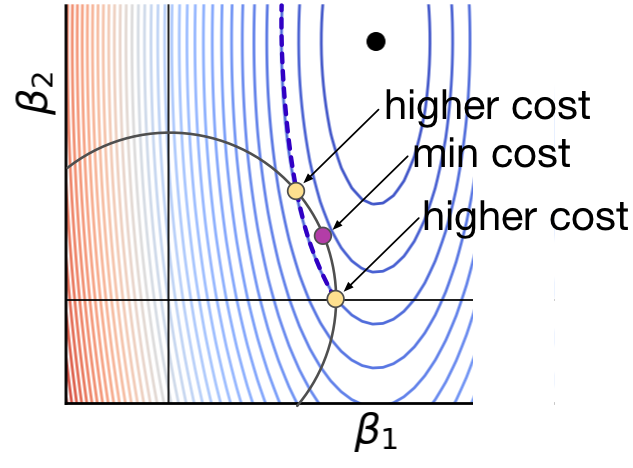
\includegraphics[width=0.45\textwidth]{images/L2contour.png}
        \hspace{1em}
        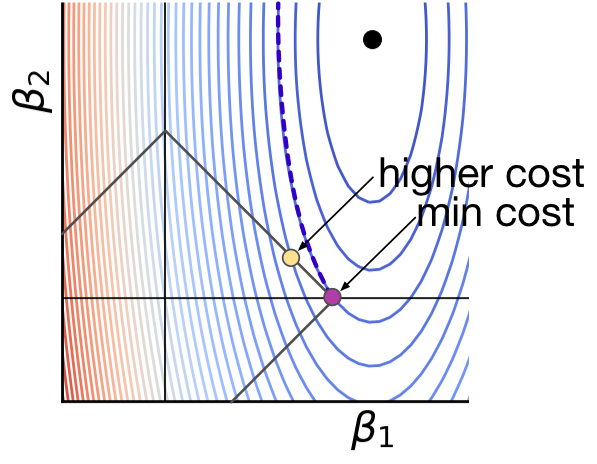
\includegraphics[width=0.45\textwidth]{images/L1contour.png}
        \caption{L1 and L2 constraint regions get different coefficient locations, on the diamond and circle, for the same loss function. Keep in mind that there are an infinite number of contour lines and there is a contour line exactly meeting the L2 purple dot.}
    \end{figure}
\end{frame}

\begin{frame}{Elastic Net: The Best of Both Worlds}
    What if you want both sparsity from L1 and the smoothing effect of L2?
    \begin{itemize}
        \item \bhighlight{Elastic Net} regularization is a hybrid approach that combines both L1 and L2 penalties.
        \item The penalty term is a simple weighted sum of the L1 and L2 norms:
            $$ R(W) = \sum_k \sum_l \beta W_{k,l}^2 + |W_{k,l}| $$
        \item It can produce sparse models like L1.
        \item It is more stable and often performs better than L1 when features are highly correlated.
    \end{itemize}
\end{frame}